\chapter{Including pages from PDFs}
\label{chap:pdfs} 

To include a PDF document, or pages from it, use something like this\footnote{See the package documentation for available options \url{ctan.uib.no/macros/latex/contrib/pdfpages/pdfpages.pdf}}: 

\verb|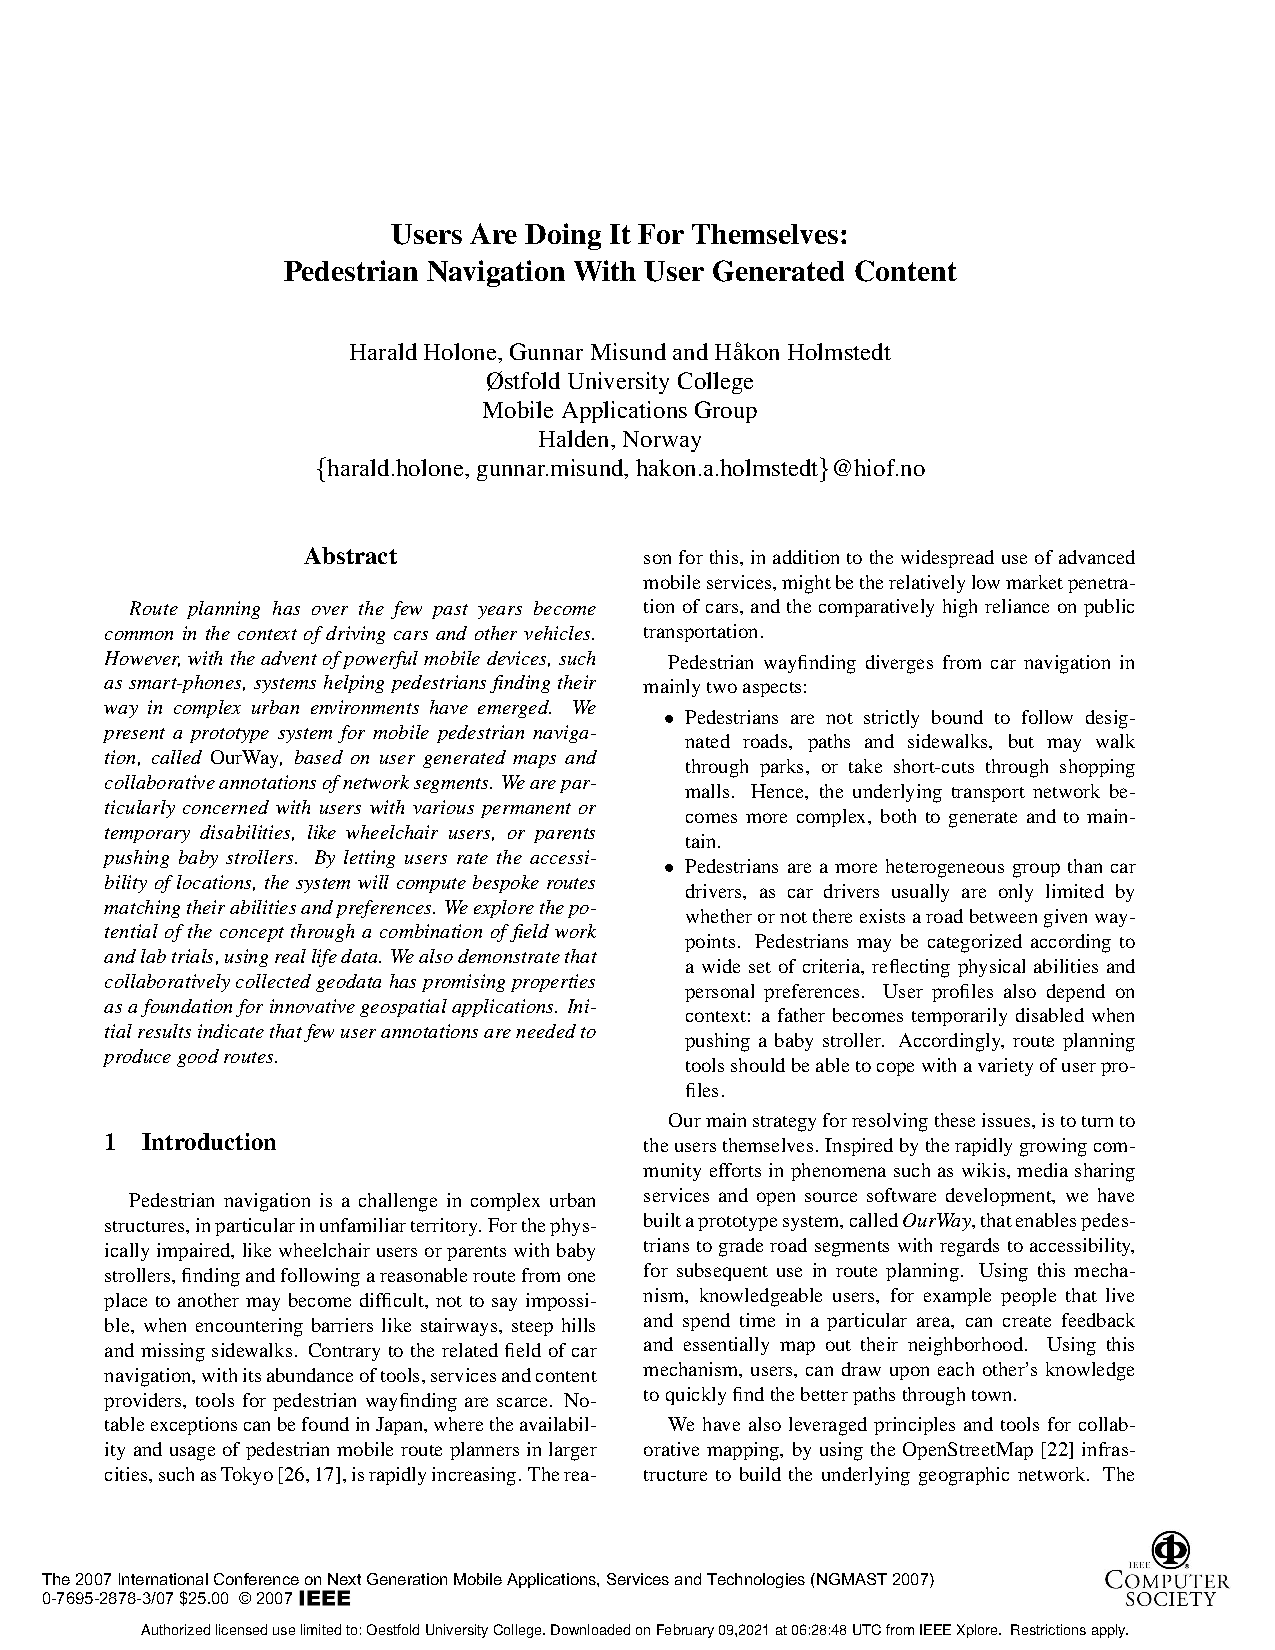
\includepdf[pages=-,pagecommand={\pagestyle{fancy}}]{Chapters/paper.pdf}|

which includes the full document, as here\parencite{holone2007users}.

To include parts of, use for example

\verb|\includepdf[pages={2,5,6},pagecommand={\pagestyle{fancy}}]{Chapters/paper.pdf}| 

or 

\verb|\includepdf[pages={3-5},pagecommand={\pagestyle{fancy}}]{Chapters/paper.pdf}|


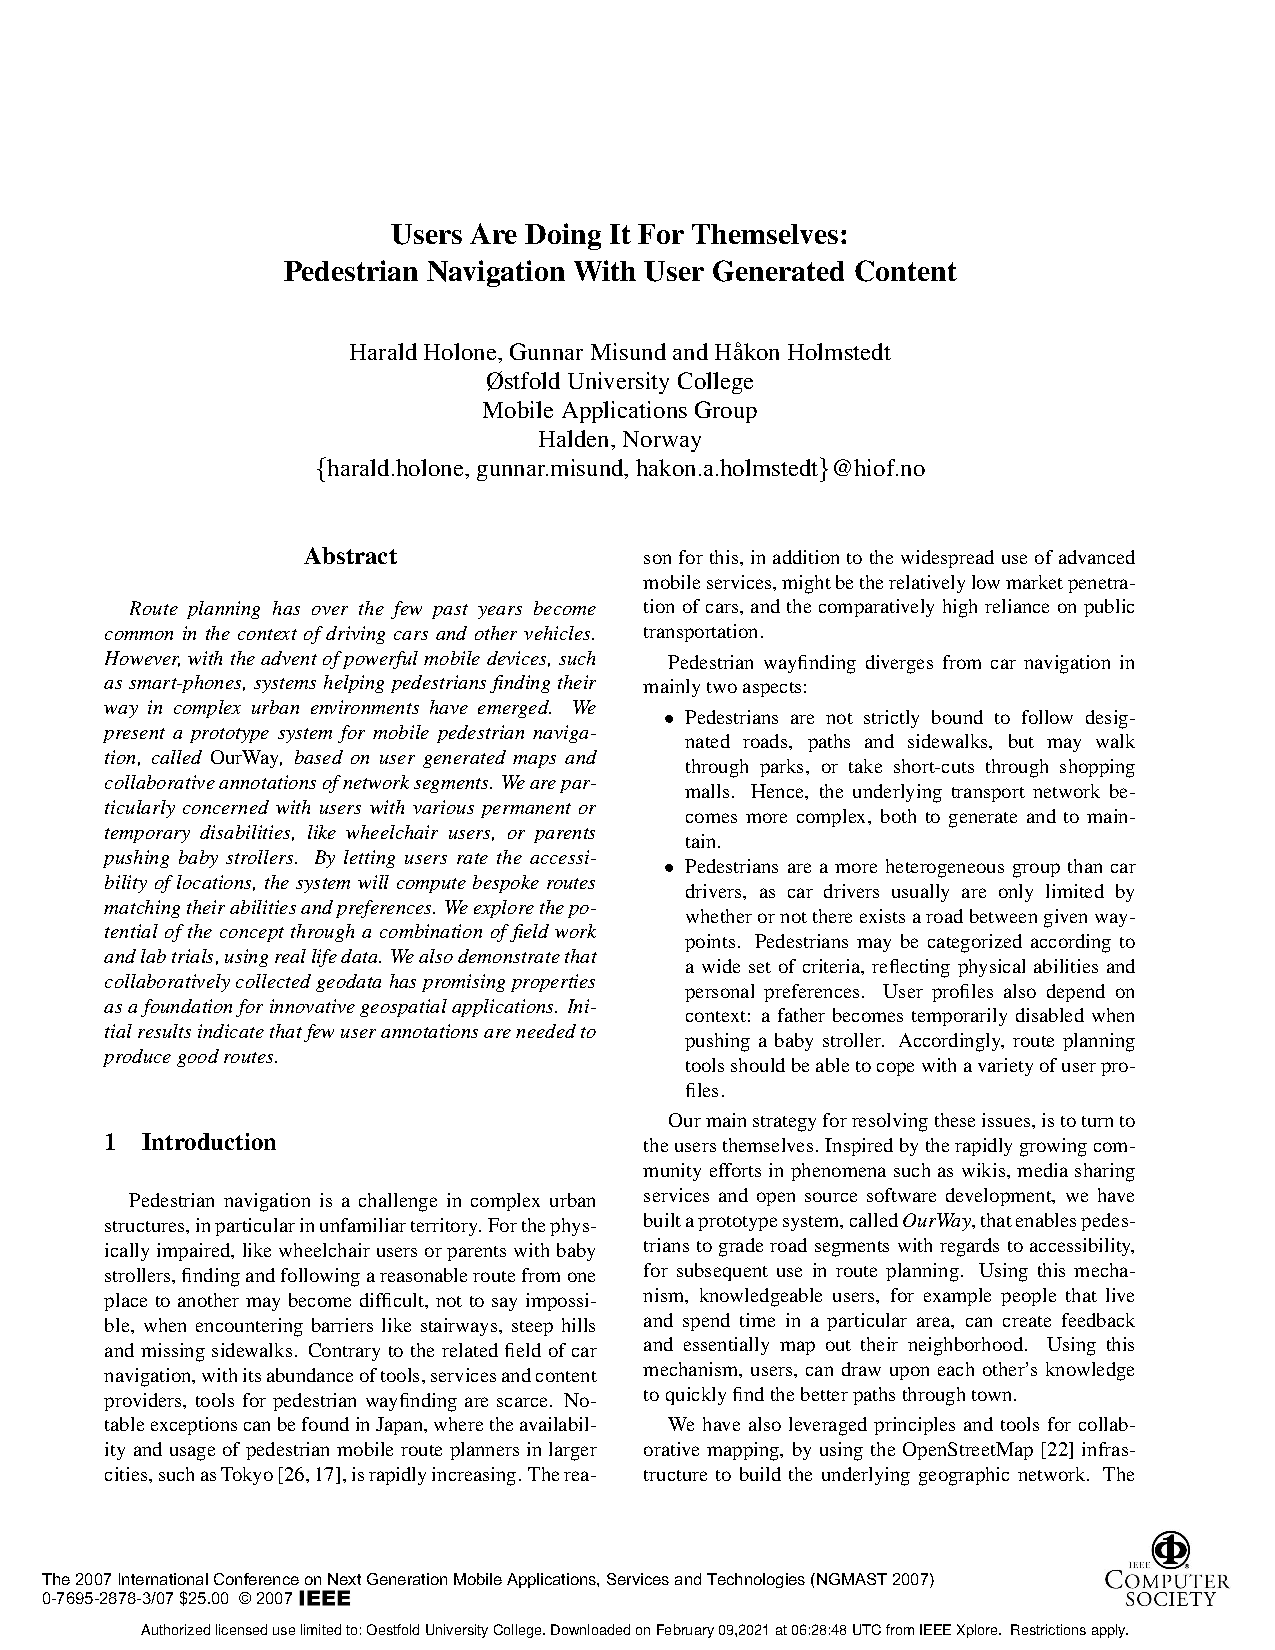
\includepdf[pages=-,pagecommand={\pagestyle{empty}}]{Chapters/paper.pdf}